\section*{Problem 4}

$x(t) = cos(200t)G_4(t)$

\subsection*{Solution}

The generic Fourier Transform for the gate function $G_\tau(t)$ is:

\begin{align}
\mathfrak{F}\{ G_\tau(t)\} &= \tau Sa\left(\frac{\omega \tau}{2}\right) \label{eq:c2p4} \\
\mathfrak{F}\{ G_4(t)\} &= 4 Sa(2 \omega) \notag
\end{align}

We can express our function as:

\begin{equation*}
x(t) = \frac{1}{2} [e^{200 t} + e^{-200 t}] G_4(t)
\end{equation*} 

As we can see from (\ref{eq:c22c}) the displacement in frecuency is reflected in the
time domain as a multiplication by an exponential. 

\begin{equation*}
X(\omega) = 2 [ Sa(2(\omega - 200)) + Sa(2(\omega + 200))]
\end{equation*} 

The plot of the magintude of $X(\omega)$ is:
\zcodemat{sources/c2p4a.m}{Plot of Magnitude}

\begin{figure}[H]
\caption{Magnitude $|X(\omega)|$}
\centering
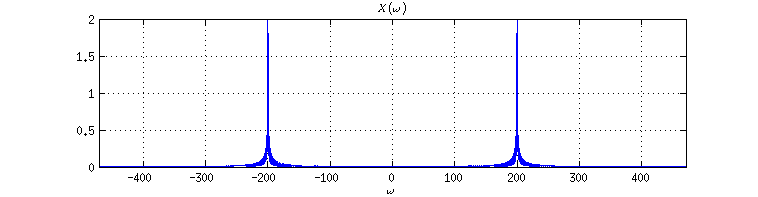
\includegraphics[width=1.0\textwidth]{figs/c2p4a.png}
\label{fig:c2p2a}
\end{figure} 

